% $ based on Id: sample_english-v1.0.tex,v 1.0 2016/10/08 21:05:22 zlb Exp $
% $Id: sample_english.tex 6 2016-10-08 13:13:33Z hsqi $

\documentclass[english]{DDCLSconf}
%\documentclass[usemulticol,english]{DDCLSconf}
\usepackage[comma,numbers,square,sort&compress]{natbib}
\usepackage{epstopdf}
\usepackage{subfigure}

\usepackage{float}
\usepackage{amsmath}%???????
\usepackage{amssymb}%?????????
\usepackage{bm}

\usepackage{diagbox} % ????
\usepackage{booktabs}
\usepackage{makecell}
\usepackage{array}
\usepackage{color}

\newcommand{\upcite}[1]{\textsuperscript{\textsuperscript{\cite{#1}}}}%上标引用 \upcite{}


\begin{document}

\title{Head Pose Estimation with Siamese Convolutional Neural Network}

\author{Fuxun Gao\aref{amss},
        Chaoli Wang\aref{amss},
%        Wu Wang\aref{hit}
}

% Note: the first argument in the \affiliation command is optional.
% It defines a label for the affiliation which can be used in the \aref
% command. If there is only one affiliation for all authors, then the
% optional argument in the \affiliation command should be suppressed,
% and the \aref command should also be removed after each author in
% \author command, in this case the affiliation will not be numbered.


\affiliation[amss]{School of Optical-Electrical and Computer Engineering, University of Shanghai for Science and Technology, Shanghai 200093, P.~R.~China
        \email{clwang@usst.edu.cn}}
%\affiliation[hit]{Harbin Institute of Technology, Harbin 150001, P.~R.~China
%        \email{xxx@hit.edu.cn}}

\maketitle

\begin{abstract}
%	Human head pose estimation has many applications in face alignment,  attention detection and behavior analysis. The conventional method for estimating the head pose is locating the facial landmarks firstly and estimate the three-dimensional pose through the facial landmarks, but the accuracy of the method depends greatly on the accuracy of the landmarks positioning. 
	In order to get rid of the dependence on keypoints and improve the accuracy of pose estimation, in this paper, we propose a method of estimating the 3D head pose using a convolutional neural network with Siamese structure. Firstly, the rank labels of head pose which used to train the Siamese network can be automatically generated from the continuous head pose labels. The Siamese network can rank the head pose deflect levels and this step is equivalent to coarse classification. Secondly, after Siamese network is trained, the continuous raw pose labels were used to fine-tuning a branch of Siamese network and let the network regress the continuous pose ground truth. For avoiding duplicate computation caused by Siamese network, we add a ensemble layer to the network. In addition, high intensity brightness adjustment and Gaussian blur are imposed on images to distort images in data augmentation, so our method will achieve perfect performances in low quality images. Experiments show that our method has higher accuracy than the state-of-the-art methods of estimating head pose from RGB images, stronger robustness than the method of head pose estimation with keypoints, and wider application range than the method of head pose estimation with depth data.
\end{abstract}

\keywords{Head Pose Estimation, Siamese, Convolutional Neural Network }

% Please remove or comment out the following line if the footnote is not necessary
\footnotetext{This work is supported by National Natural Science
Foundation (NNSF) of China under Grant  3214302006.}

\section{Introduction}

\begin{figure*}
	\centering
	
	\includegraphics[width=0.99\textwidth]{fig1.eps}
	
	% figure caption is below the figure
	
	\caption{The model architecture of head pose estimation with Siamese neural network. }
	
	\label{model}       % Give a unique label
\end{figure*}	

Human head pose estimation is a key technology in face recognition, face alignment, attention detection, behavior analysis and other applications. Current face recognition technology has a high recognition accuracy of 99.82\% for frontal faces\upcite{lightcnn}. However, as the face pose angle increase, the accuracy of face recognition decreases. Therefore, it's necessary to filter out large-angle faces that are not conducive to recognition before face recognition with head pose estimation. The head pose generally reflects the gaze direction of the human eye, and can be used as a method of attention detection for driver attention detection, fatigue driving detection, and behavior analysis in assisted driving \upcite{driver}.

At present, the method of human head pose estimation is mainly classified into three types according to the type of data used: RGB image, depth data, and a combination of RGB image and depth data. Using depth data or using depth data combined with RGB images\upcite{siamese_depth} to estimate the human head posture angle is more accurate, but relying on the depth camera or binocular camera to measure depth data. The cost of equipment is expensive and those cameras were greatly affected by illumination and other environment. The application scope of head pose estimation with depth information is limited. Nevertheless, head pose estimation with RGB images only rely on monocular camera, this method has advantage of low cost and wide application range, whereas the accuracy is lower than the method with depth information.

The conventional head pose estimation approach with RGB images is establishing the face appearance model by the facial landmarks, the three-dimensional posture of the face is calculated by the geometric relationship between the established face model and the standard face appearance template model \upcite{AAM,keypoint,fan,dlib,video}. The optimization direction of this method is to improve the accuracy of facial landmarks positioning. To extract accurate facial landmarks, \cite{AAM} uses statistical modeling methods to model the texture and shape statistical and locate the keypoints, but this method has low precision and poor generalization. Convolutional neural networks have become ubiquitous in the field of computer vision since AlexNet \upcite{alexnet} made a breakthrough in the ImageNet Competition in 2012, and \cite{keypoint} acquired more accurate facial landmarks coordinates with convolutional neural networks. However, the method of calculating the pose angle of head through the keypoints depends on the accuracy of the keypoint positioning, the calculated pose angle will produce a large error when the keypoints are	difficult to locate in distorted images.

In order to get rid of the dependence on keypoints, numerous scholars have devoted themselves to directly predicting the three-dimensional pose of the human head through RGB images with deep learning. The conventional approach is directly regressing the specific values of the three-dimensional head pose with the convolutional neural network. For example, \cite{direct_regression} uses convolutional neural network architecture which designed by themselves to fit the three-dimensional head pose with RGB images. However, on the one hand, this kind of continuous labels are difficult to fit and it's impossible to achieve satisfactory results when the amount of data is limited. On the other hand, their method does not make full use of the existing high-performance network architecture, such as VGG \upcite{vgg}, Inception \upcite{inception}, ResNet \upcite{resnet} and them like, this also limits the performance of their method.

For the sake of acquiring accurate 3D head pose angle, Ruiz N et al. propose a multi-loss convolutional neural network called HopeNet \upcite{hopenet}, which transforms the regression of pose angle into a combination of classification and regression, and reduces the difficulty of pose regression by classification. The HopeNet uses ResNet50 as the backbone network, and two loss functions are designed. One uses the cross entropy loss to roughly classify the head pose angle, the another uses the mean square error loss to regress the specific value of the head pose, and the optimization goal is the weighted sum of the two losses, consequently, the network regresses pose from coarse to fine. This method yields better results than the direct regression method. However, the general head pose datasets have the problem of serious data distribution imbalances. There are a large number of small-angle pose data, but there are very few large-angle pose data, which will greatly affect HopeNet's classification loss and affect regression loss to some extent. In addition, \cite{quatnet} also propose a head pose estimation with multi-regression loss like HopeNet called QuatNet and achieve great performance.

For solving the severe problem of data distribution imbalance on the dataset, narrowing the gap between the method of directly predicting the head pose from the RGB images and the method of calculating the head pose with the depth information, as is shown in Fig.\ref{model}, we proposed a method for estimating the 3D pose of the human head with the Siamese network structure \upcite{siamese}. This method is mainly divided into three steps:
 
Step1: Generate the rank labels from the continues row pose label automatically. For example, the pose angle is divided by an interval of 3 degrees, and the angle within the interval belongs to the same rank level. 

Step2: Feed pairs of images and corresponding pose rank labels into the Siamese network. The Siamese network will compare paired images to rank the pose angles instead of categorizing pose angle like HopeNet. Ranking is less affected by the data distribution imbalance than classification and contain more information, so it will get better results. 

Step3: Fine-tuning a branch of the Siamese network with the raw pose labels, so the network can inference the specific pose value. 

In addition, in order to improve the generalization of our method, high-intensity Gaussian noise, motion blur and image brightness adjustment are applied during data augmentation, so that our method can get excellent performance in low-quality images and have a widely application scope. The effects of our method proposed in this paper under different environments are shown in Fig.\ref{result_in_different_envs}.

The major contributions of our method are summarized as follows:
\begin{enumerate}
	\item On the one hand, our method improves the accuracy of pose estimation from RGB images, narrows the gap between the methods of estimating head pose from depth information and RGB images. On the other hand, our method gets rid of the dependence on facial landmarks and has stronger robustness.
	\item Siamese network is used to compare and rank images rather than classify them like HopeNet, which reduces the impact of data distribution imbalance in train set and improves the performance of the network.
	\item The structure of Siamese network is improved by adding ensemble layer before loss layer, which can avoid the repeated calculation and accelerate the operation speed.
	\item High-intensity disturbance are imposed during data augmentation to reduce image quality, so our method can achieve better performance on low-quality images.
\end{enumerate}

\section{Head Pose Estimation}
%In this section, the method proposed in this paper will be introduced, including how to use the Siamese network to rank the 3D pose of the human head, how to improve the Siamese network to avoid repeat compute, how to fine-tuning the model, which kind of loss function to choose and the information about train set and test set and so on.

\subsection{Improve Siamese Network}

The standard Siamese network has two backbone network branches but sharing single loss function, which is widely used in identification, tracking and so on. The backbone networks in the two branches share weights, the paired images and the corresponding labels are fed into the Siamese network. The paired images through different branches produce an output respectively, then the outputs of the two branches are fed into the loss layer to compare the two images. The gradient of the loss layer is propagated back to two branches, so the parameters are updated. But due to each image is fed into two branches, the amount of calculation will increase sharply.  


\begin{figure}[!htb]
	\centering
	
	\includegraphics[width=0.49\textwidth]{fig2.eps}
	
	% figure caption is below the figure
	
	\caption{The standard Siamese network (left) and the improved Siamese network (right).}
	
	\label{siamese}       % Give a unique label
	
\end{figure}		

As described in Fig.\ref{siamese}, to reduce the the computation of Siamese network, we remove a branch of the Siamese network and add a ensemble layer before the loss layer. When a batch of images are fed into the Siamese network, their feature maps of different rank level extracted by the backbone network will be paired in the ensemble layer and then passed to the loss layer. The ensemble layer just pair images of different rank level without additional computations for the network. This improvement can avoid repeated feature extraction in backbone network but it can achieve the same effect as the Siamese network.

Suppose there are $n$ images of different pose rank levels, if the standard Siamese network are used to compare different levels of images, we need to feed about $n^{2}-n$ images into the network. However, if we use our improved efficient Siamese network to complete the same task, the backbone network only need to extract the feature maps once from the $n$ images, then the task of match feature maps of different levels images is performed in the ensemble layer. There is no process of repeated computation in the improved Siamese network which will not wastes computing resources, and the time for extracting features of the network can be accelerated by $\frac{n^2-n}{n}=n-1$ times. The convergence curves of picth angle ranking loss on 300W-LP dataset for our improved Siamese network versus the standard Siamese network are shown in Fig.\ref{siamese_curves}.
\begin{figure}[!htb]
	\centering
	
	\includegraphics[width=0.4\textwidth]{fig3.eps}
	
	% figure caption is below the figure
	
	\caption{Comparison between the standard Siamese network and our improved Siamese network in pitch angle.}
	
	\label{siamese_curves}       % Give a unique label
	
\end{figure}

\subsection{Loss Function}
Since the purpose of the Siamese network is ranking the pose angles of the human head in the images, the output of the network is a discrete value and the value represents a coarse range of head pose angles in the images. The loss function of the Siamese network is the pairwise ranking binary cross entropy loss. If the paired images are represented as $x$ and the predicted value of the Siamese network is represented as $p$, the ground truth is $y$, then the binary cross entropy loss $L$ can be noted as 
\begin{equation}
L\left ( x_i,\ y_i \right )=-\left [ y\cdot log\left ( p \right ) +\left ( 1-y \right ) \cdot log\left ( 1-p \right ) \right ]
\end{equation}
Here, $x$ represents a pair of images and as the input of Siamese network. If two images belong to the same head pose rank level, the ground truth $y$ is $1$, else $y$ is $0$.

\subsection{Fine-tuning for Head Pose}
After training the Siamese network for ranking the head pose, we remove the ensemble layer of the improved Siamese network and use the pre-trained model in Siamese network to initialize the network, then we use the continuous raw pose labels of the dataset to fine tune the network for fine-grained regression. This is equivalent to using one of the Siamese network branches to regress the head pose. In general, the rank job in Siamese network is a coarse regression and this step is fine-grained head pose estimation.

The loss function of regression is the minimum mean-square error (MSE):
\begin{equation}
L\left ( y_i,\hat{y}_i \right )=\frac{1}{n}\sum_{i=1}^{n}\left ( y_i-\hat{y}_i \right )^2
\end{equation}
Where $n$ is the batch size, $y_i$ is the pose ground truth of the $i$-th image and the predict value of the $i$-th image is $\hat{y}_i$.

After fine-tuning the network, the network can directly inference the specific values of the 3D head pose, and complete the end-to-end head pose estimation.

\subsection{Dataset}
The dataset used for training is 300W-LP \upcite{300w-lp}, which is a synthetic face dataset with approximately 122,450 images. A face model is fit on each image and the image is distorted to vary the yaw of the face which gives us pose across several yaw angles. The retained 2D keypoints are used to relabel the head pose angle. The dataset contains the accurate head pose value of yaw, pitch and roll. Because of the information of the 3D model of each face and the angle of 6 degrees of freedom in each image are exists, the pose angle labels are very accurate. 

Due to the large deflection of the face in yaw direction and the small deflection in the pitch and roll directions in real life, the dataset is only focused on the uniform distribution of the yaw direction. Fig.\ref{300w-lp} shows the head pose data distribution of the synthesized dataset 300W-LP. It can be seen that the yaw angle distribution is relatively balance, but the pitch and roll angles are largely concentrated in the bins of $[23, 38]$, that is, within the $[-30^{\circ}, 21^{\circ}]$ angle range.

The test set is AFLW2000, the entire dataset has 2000 identities and each identity has one image. Each image in the dataset is labeled with 68 3D facial landmarks and precise face 3D pose annotations. The dataset contains images that captured in different backgrounds and different illumination environments, undoubtedly, it's similar to the real application scene. Due to numerous identities and a number of large deflection angle images in this dataset, we select this dataset as our test set. The data distribution of AFLW2000 is shown in Fig.\ref{aflw2000}.


\begin{figure}[!htb]
	\centering
	
	\subfigure[300W-LP]{\label{300w-lp}
		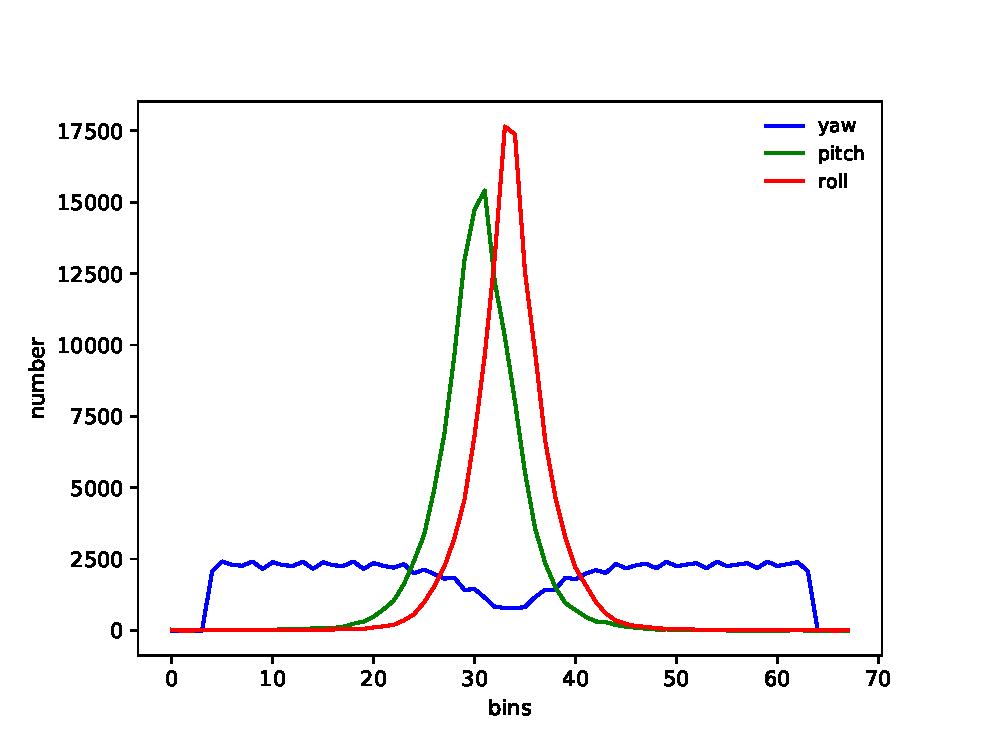
\includegraphics[width=0.325\textwidth]{fig4a.eps}
	}
	\subfigure[ALFW2000]{\label{aflw2000}
		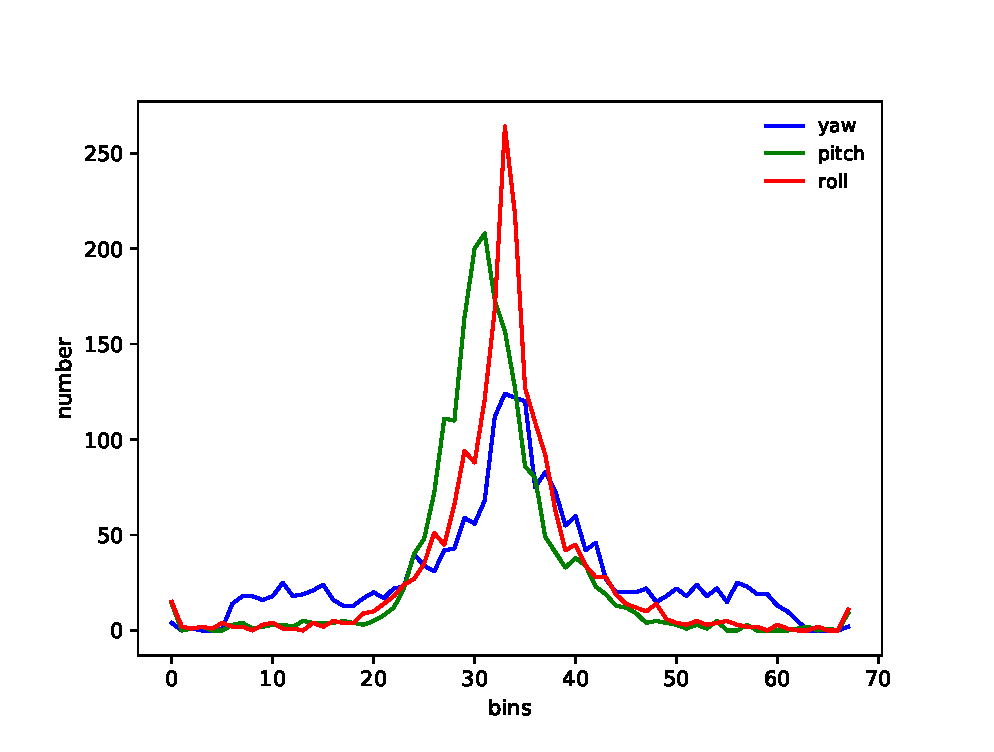
\includegraphics[width=0.325\textwidth]{fig4b.eps}
	}
	
	\caption{Data distribution: $bins$ represents the rank labels that divide the head pose $[-99^{\circ}, 99^{\circ}]$ into different intervals, the pose angle within the 3 degree belong to the same level. We can use $bin\times 3-99^{\circ}$ to get the coarse angle that the $bin$ represent. The $number$ represent the number of images in this $bin$.}
	\label{data_distribution}       % Give a unique label
	
\end{figure}

\subsection{Robustness on Low-quality Images}
Compared to the method of head pose estimation with keypoints, our method is more robust on low-quality images. If the head images are distorted, the accuracy of keypoints positioning will drop dramatically, and the performance of head pose estimation will be seriously affected. To overcome the weakness, in our method, we impose high-intensity brightness adjustment on images in data augmentation to enhance the performance of our method in dark or brightness environment. We impose high-intensity Gaussian blur on the training image to enhance the robustness of our algorithm in the blurred image. In addition, in order to improve the accuracy of head pose estimation in the obscured face images, we resize the head images to $300\times 300$ firstly, then the random crop is used to crop the size of $224\times 224$ image patches as the input of our network. These measures improve the robustness of our approach in different images, the effects of our approach in low-quality images are shown in Fig.\ref{result_in_different_envs}.

\begin{figure}[!htb]
	\centering
	\subfigure{
		\includegraphics[width=0.22\textwidth]{fig5a.jpg}
		%\caption{fig1}
	}
	\subfigure{
		\includegraphics[width=0.22\textwidth]{fig5b.jpg}
	}
	\quad
	\subfigure{
		\includegraphics[width=0.22\textwidth]{fig5c.jpg}
	}
	\subfigure{
		\includegraphics[width=0.22\textwidth]{fig5d.jpg}
	}
	\caption{The performance of our method in different images such as large pose angle (upper left), face occlusion (upper right),  dark light (lower left) and blurred images (lower right) and them like. The blue, red and green axis in the images point towards the front, the right side and the downward of the head respectively.}
	\label{result_in_different_envs}
\end{figure}

\section{Experiments and Results}
The method proposed in this paper need Siamese network to rank the head pose angle firstly. This step is equivalent to coarse classification of the head pose, but the Siamese network rank the images by contrasting paired images when train the Siamese network, instead of classify the head pose angle like HopeNet. Ranking contains more information than the classification, which can avoid the influence of the imbalance distribution of the dataset.

In order to rank the head pose, we need a rank label that generate from the raw continues pose labels automatically. The three-dimensional pose angles of yaw, pitch, and roll in the 300W-LP dataset are mainly distributed in $[-99^{\circ}, 99^{\circ}]$, so it is reasonable to divide $3^{\circ}$ into  one rank level. In addition, we use three separate losses and on for each angle as is shown in Fig.\ref{model}. In order to compare with HopeNet, we choose the ResNet50 as our backbone to extract the feature map and three separate fully-connected layers are used to predict the yaw, pitch and roll angles. The losses of the three directions are used to update the parameters in the backbone and the three separate fully-connected layers.

Adam optimization is selected as the optimizer, where $\beta _1=0.9$, $\beta _2=0.999$, $\epsilon =10^{-8}$, the initial learning rate is $10^{-3}$ and decreases with the increase of iteration steps. The pre-trained model in ImageNet is used to accelerate the convergence of our network. 

After the Siamese ranking network is trained, the network without the ensemble layer is initialized with the weights obtained from the Siamese network, the loss function is replaced by the mean square error. We use the raw pose label in 300W-LP to fine-tune the network, so that the network can output the specific head pose value.
\begin{figure}[!tbp]
	\centering
	
	\includegraphics[width=0.43\textwidth]{fig6.jpg}
	\caption{Loss function curve of direct regression method.}	
	\label{loss1}       % Give a unique label	
\end{figure}
\begin{figure}[!tbp]
	\centering
	\includegraphics[width=0.43\textwidth]{fig7.jpg}
	\caption{Loss function curve of HopeNet.}	
	\label{loss2}       % Give a unique label
	
\end{figure}
\begin{figure}[!tbp]
	\centering	
	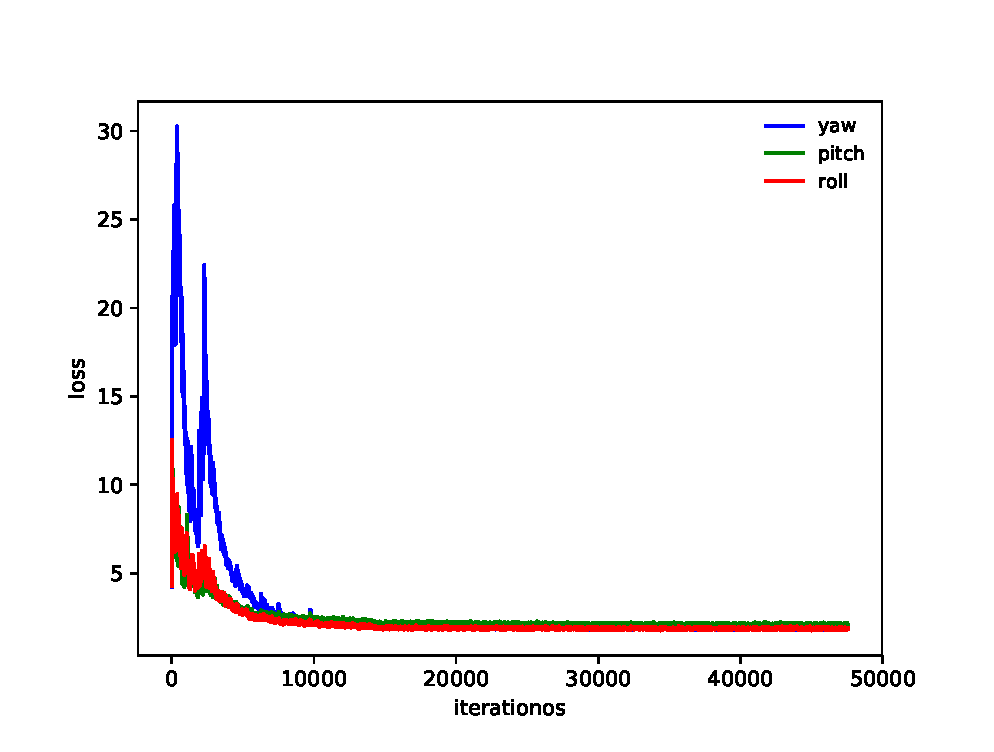
\includegraphics[width=0.43\textwidth]{fig8.eps}
	\caption{Loss function curve of our method.}	
	\label{loss3}       % Give a unique label	
\end{figure}
%\begin{figure}[!tbp]%[H]????
%	\centering
%	\subfigure[Regression directly]{\label{reg_loss}
%		\includegraphics[width=0.22\textwidth]{./figs/fig6a.jpg}
%		%\caption{fig1}
%	}
%	\subfigure[HopeNet]{\label{hopenet_loss}
%		\includegraphics[width=0.22\textwidth]{./figs/fig6b.jpg}
%	}
%	%	\quad
%	\subfigure[Our Method]{\label{our_loss}
%		\includegraphics[width=0.22\textwidth]{./figs/fig6c.eps}
%	}
	
%	\caption{The loss convergence curve of different methods.}
%	\label{loss}
%\end{figure}

Fig.\ref{loss1} is the loss curve that use ResNet50 to regress the head pose directly. It can be seen that the loss function fluctuates greatly and the yaw angle can convergence to a very low value, but loss of the pitch and roll angle cannot converge to the same level due to the data distribution is imbalance. Fig.\ref{loss2} is the loss curve of HopeNet.
Compared with Figure 1, the loss of HopeNet converges faster and smoothly, because HopeNet use classification to reduce the difficulty of regression. Our method's loss curve is shown in Fig.\ref{loss3}. The loss of yaw, pitch and roll can convergence to the same level because we use the Siamese network to rank head pose instead of categorizing angles like HopeNet. Ranking contains more information than the classification, which can reduce the influence of the imbalance distribution of the dataset.

Our method can overcome the influence of data distribution imbalance to a certain extent, and can obtain more accurate angle value in large angle deflection images than HopeNet. The evaluation metric is Mean Absolute Error (MAE), which is the same as that in HopeNet. 
\begin{equation}
MAE = \frac{1}{n}\sum_{i=1}^{n}\left | y_i-\hat{y}_i \right |
\end{equation}
Where $n$ is the number of test images, $y_i$ is the head pose angle of the $i$-th image that predicted by the network, and $\hat{y}_i$ is the ground truth of the $i$-th image.

The results of our method and other state-of-the-art methods on ALFW2000 dataset are shown in Fig.\ref{result_compare}. Where Patacchiola M\upcite{direct_regression} directly regress the three-dimensional head pose with convolution neural network. HopeNet uses multi-loss cascade method to complete the same task. FAN\upcite{fan} uses 12 keypoints of human face for head pose estimation and 3DMM\upcite{3DMM} uses depth information for head pose estimation. We can see that 3DMM is the most accurate and robust method in head pose estimation, because the depth information is used in this method. HopeNet make tremendous progress compared with Patacchiola M's directly regression method, futhermore, our method achieve better performance than HopeNet, in addition, the robustness and accuracy of our method are better than those of FAN.

\begin{figure}[!tbp]
	\centering
	
	\includegraphics[width=0.49\textwidth]{fig9.eps}
	\caption{Result compare of different method.}
	
	\label{result_compare}       % Give a unique label
	
\end{figure}

The effect of head pose estimation with depth information is best. Head pose estimation with keypoints is dependent on the accuracy of keypoints position and the number of keypoints used. But the effect of the keypoints' locate accuracy will decrease as the number of keypoints used to head pose estimation increase. The direct regression method cannot achieve the satisfactory result. The multi-loss approach proposed in HopeNet can generally reduce the error of head pose estimation, however, as shown in Table \ref{different_pose_compare}, HopeNet is very accurate for pose estimation at small angles, but the performance of pose estimation at large angles decreases dramatically. But our method performs well in both large and small angles. The reason is that the cascade loss include the classification which greatly influenced by the data distribution imbalance. The method proposed in this paper transforms the classification in HopeNet to rank, which contains more information than classification. The improvement can reduce the impact of data distribution imbalance and improve the robustness of the model.


\begin{table*}[!tbp]
	% table caption is above the table
	\caption{Comparison of MAE of different methods at different pose angles range.}
	\label{different_pose_compare}       % Give a unique label
	\centering
	\begin{tabular}{ccccccc}
		\toprule
		\quad & \quad & Patacchiola M & HopeNet & FAN & 3DMM & Our method\\
		\midrule
		Yaw & $[0^{\circ}, 30^{\circ})$ & 6.223 & 2.690 & 2.579 & 2.331 & 5.531 \\
		\quad & $[30^{\circ}, 60^{\circ})$ & 9.187 & 12.892 & 6.294 & 2.657 & 6.751 \\
		\quad & $[60^{\circ}, 99^{\circ}]$ & 15.890 & 18.650 & 24.001 & 2.519 & 8.920 \\
		
		Pitch & $[0^{\circ}, 30^{\circ})$ & 6.581 & 2.487 & 4.783 & 2.634 & 5.481 \\
		\quad & $[30^{\circ}, 60^{\circ})$ & 10.692 & 17.502 & 9.989 & 1.155 & 7.690 \\
		\quad & $[60^{\circ}, 99^{\circ}]$ & 15.988 & 25.507 & 34.273 & 1.979 & 10.690 \\
		
		Roll & $[0^{\circ}, 30^{\circ})$ & 6.149 & 2.952 & 3.589 & 1.668 & 5.483 \\
		\quad & $[30^{\circ}, 60^{\circ})$ & 12.859 & 11.910 & 6.576 & 2.103 & 6.613 \\
		\quad & $[60^{\circ}, 99^{\circ}]$ & 16.943 & 21.572 & 38.237 & 2.436 & 12.127 \\
		
		\bottomrule
	\end{tabular}
\end{table*}


\section{Conclusion}
The proposed method of head pose estimation with Siamese can greatly improve the accuracy of angle regression compared to HopeNet and other methods, especially in the large angle deflected head images. In addition, we improves the Siamese network and designs a ensemble layer, which can use a single backbone network to achieve the same effect as the standard Siamese network. Furthermore, we use a variety of methods to distort images in data augmentation so that our method can achieve better performance on low-quality images. Experiments prove that our method improves the performance of head pose estimation in RGB images. Our approach narrows the gap with the accurate methods which use the depth information to estimate the head pose and has stronger robustness compare with conventional method with keypoints. Of course, there is still a wide gap between our method and the method with depth information in human head pose estimation. This will constantly inspire us to keep exploring.


\begin{thebibliography}{0}
\balance	
\bibitem{lightcnn} Wu X, He R, Sun Z, et al. A light CNN for deep face representation with noisy labels[J]. \emph{IEEE Transactions on Information Forensics and Security}, 2018, 13(11): 2884-2896.

\bibitem{driver} Schmied R , Obereigner G , Waschl H . Analysis and Adaptive Estimation of Human Car Following Behavior for Advanced Driver Assistance Systems[C]//\emph{ Wcx 17: Sae World Congress Experience}. 2017.%DDCLS17  ?????????

\bibitem{siamese_depth} Venturelli M, Borghi G, Vezzani R, et al. From depth data to head pose estimation: a siamese approach[J]. \emph{arXiv preprint arXiv:1703.03624}, 2017.%siamese

\bibitem{AAM} Cootes T F, Edwards G J, Taylor C J. Active appearance models[J]. \emph{IEEE Transactions on Pattern Analysis \& Machine Intelligence}, 2001 (6): 681-685. %

\bibitem{keypoint} Kumar A, Alavi A, Chellappa R. Kepler: Keypoint and pose estimation of unconstrained faces by learning efficient h-cnn regressors[C]//\emph{Automatic Face \& Gesture Recognition (FG 2017), 2017 12th IEEE International Conference on}. IEEE, 2017: 258-265. %

\bibitem{fan} Bulat A, Tzimiropoulos G. How far are we from solving the 2d \& 3d face alignment problem?(and a dataset of 230,000 3d facial landmarks)[C]//\emph{International Conference on Computer Vision}. 2017, 1(2): 4.%fan

\bibitem{dlib} Kazemi V, Sullivan J. One millisecond face alignment with an ensemble of regression trees[C]//\emph{Proceedings of the IEEE Conference on Computer Vision and Pattern Recognition}. 2014: 1867-1874.%dlib:

\bibitem{video}C.~Yu. A Fast Algorithm for Face Pose Estimation in Video Image[J]. \emph{Modern Computer}. 2018, No.612(12):48-50+55.

\bibitem{alexnet} Krizhevsky A, Sutskever I, Hinton G E. Imagenet classification with deep convolutional neural networks[C]//\emph{Advances in neural information processing systems}. 2012: 1097-1105. %AlexNet

\bibitem{direct_regression} Patacchiola M, Cangelosi A. Head pose estimation in the wild using convolutional neural networks and adaptive gradient methods[J]. \emph{Pattern Recognition}, 2017, 71: 132-143.%

\bibitem{vgg} Simonyan K, Zisserman A. Very deep convolutional networks for large-scale image recognition[J]. \emph{arXiv preprint arXiv:1409.1556}, 2014.

\bibitem{inception} Szegedy C, Liu W, Jia Y, et al. Going deeper with convolutions[C]//\emph{Proceedings of the IEEE conference on computer vision and pattern recognition}. 2015: 1-9.%inception-v1

\bibitem{resnet}He K, Zhang X, Ren S, et al. Deep residual learning for image recognition[C]//\emph{Proceedings of the IEEE conference on computer vision and pattern recognition}. 2016: 770-778.%resnet

\bibitem{hopenet} Ruiz N, Chong E, Rehg J M. Fine-Grained Head Pose Estimation Without Keypoints[J]. \emph{arXiv preprint arXiv:1710.00925}, 2017.% hopenet

\bibitem{siamese} Bromley J, Guyon I, LeCun Y, et al. Signature verification using a ``siamese" time delay neural network[C]//\emph{Advances in neural information processing systems}. 1994: 737-744.%siamese network

\bibitem{quatnet} Hsu H W, Wu T Y, Wan S, et al. QuatNet: Quaternion-based Head Pose Estimation with Multi-regression Loss[J]. \emph{IEEE Transactions on Multimedia}, 2018.%quatnet:

%\bibitem{RankIQA} Liu X, van de Weijer J, Bagdanov A D. Rankiqa: Learning from rankings for no-reference image quality assessment[J]. \emph{Computer Vision and Pattern Recognition}, 2017.%RankIQA

\bibitem{300w-lp} Zhu X, Lei Z, Liu X, et al. Face alignment across large poses: A 3d solution[C]//\emph{Proceedings of the IEEE conference on computer vision and pattern recognition}. 2016: 146-155. %300w-lp???

\bibitem{3DMM} Yu Y, Mora K A F, Odobez J M. Robust and accurate 3d head pose estimation through 3dmm and online head model reconstruction[C]//\emph{Automatic Face \& Gesture Recognition (FG 2017), 2017 12th IEEE International Conference on}. IEEE, 2017: 711-718.%

%\bibitem{omnidirectional_camera_cnn} Yamaura Y, Tsuboshita Y, Onishi T. Head Pose Estimation for an Omnidirectional Camera Using a Convolutional Neural Network[C]//\emph{2018 IEEE 13th Image, Video, and Multidimensional Signal Processing Workshop (IVMSP)}. IEEE, 2018: 1-5.%








	
%\bibitem{cheng2005}
%D.~Cheng, Controllability of switched bilinear systems, \emph{IEEE Trans. on
%  Automatic Control}, 50(4): 511--515, 2005.
%
%\bibitem{poor1985}
%H.~Poor, \emph{An Introduction to Signal Detection and Estimation}. New York: Springer-Verlag, 1985, chapter 4.
%
%\bibitem{smith}
%B.~Smith, An approach to graphs of linear forms, accepted.
%
%\bibitem{cheng2005a}
%D.~Cheng, On logic-based intelligent systems, in \emph{Proceedings of 5th
%  International Conference on Control and Automation}, 2005: 71--75.
%
%\bibitem{cheng2005b}
%D.~Cheng, R.~Ortega, and E.~Panteley, On port controlled hamiltonian systems,
%  in \emph{Advanced Robust and Adaptive Control --- Theory and Applications},
%  D.~Cheng, Y.~Sun, T.~Shen, and H.~Ohmori, Eds. Beijing: Tsinghua University Press, 2005: 3--16.

\end{thebibliography}

\end{document}
